\documentclass[a4paper,11pt,oneside]{scrreprt}
\usepackage[latin1]{inputenc}
\usepackage[english]{babel}
\usepackage{graphicx}
\usepackage{float}
\usepackage{geometry}
\geometry{verbose,a4paper,tmargin=25mm,bmargin=25mm,lmargin=15mm,rmargin=25mm}
\usepackage{paralist}

\usepackage{paracol}

\usepackage{todonotes}

\usepackage{listings}
\lstset{language=Java,
	tabsize=2,
	showspaces=false,
	showtabs=false,
	breaklines=true,
	showstringspaces=false,
	breakatwhitespace=true,
	commentstyle=\color{pgreen},
	keywordstyle=\color{pblue},
	stringstyle=\color{pred},
	basicstyle=\footnotesize\ttfamily,
	moredelim=[il][\textcolor{pgrey}]{$$},
	moredelim=[is][\textcolor{pgrey}]{\%\%}{\%\%}
}

\usepackage{tikz}
\usetikzlibrary{calc,patterns,angles,quotes}

\usepackage{caption}
\usepackage{subcaption}
\usepackage{tabularx} % in the preamble

\begin{document}


\begin{center}
	Submitted by Group 51
	
	\bigskip
	
	\begin{tabular}{c}
	Group Members: \\
	CETIN, Ulfet (391819); GRUCZKA, FILIP (413279);	LIPINSKI, Bartosz (413177) \\
	\end{tabular}

	\bigskip
	
	DIS1 WS 19/20 Assignment 2\\
	Applying Design Principles to Evaluate and Redesign UIs
	
	%	(ordered on lastname basis)
\end{center}

\section*{Task 1}

%\begin{figure}[h]
%	\centering
%	\includegraphics[clip, trim=0cm 7cm 29cm 0cm, scale=0.5]{./images/bad1st.png}
%	\includegraphics[clip, trim=0cm 113cm 29cm 0cm, scale=0.5]{./images/bad2nd.png}
%\end{figure}
%

%\begin{figure}[H]
%	\centering
%	\begin{subfigure}{.5\textwidth}
%		\centering
%		\includegraphics[clip, trim=0cm 7cm 25cm 0cm, scale=0.5]{./images/bad3.png}
%%		\caption{A subfigure}
%		\label{fig:sub1}
%	\end{subfigure}%
%	\begin{subfigure}{.5\textwidth}
%		\centering
%		\includegraphics[clip, trim=-2cm 7cm 25cm 0cm, scale=0.50]{./images/bad1.png}
%%		\caption{A subfigure}
%		\label{fig:sub2}
%	\end{subfigure}
%	\caption{Paul Graham website}
%	\label{fig:test}
%\end{figure}

\begin{figure}[H]
	\centering
	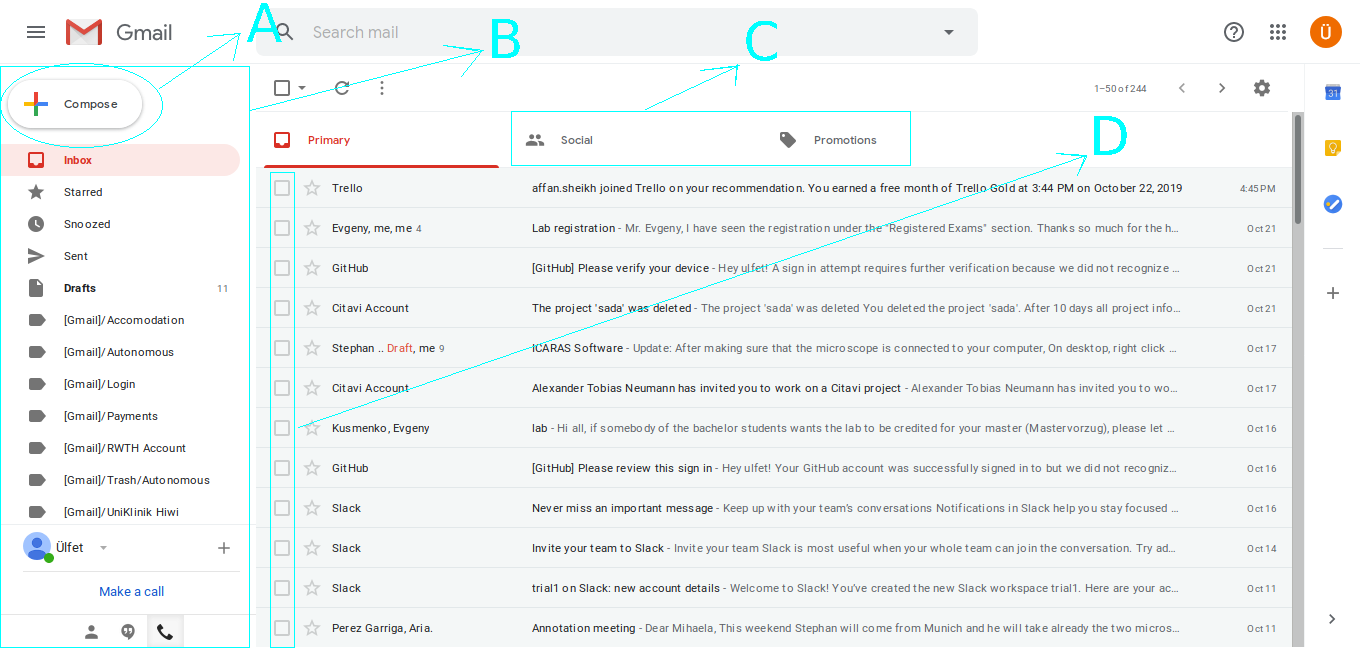
\includegraphics[clip, trim=0cm 1cm 0cm 0cm, scale=0.33]{./images/gmail1.png}
	\caption{Gmail}
	\label{fig:sub2}
\end{figure}

\begin{figure}[H]
	\centering
	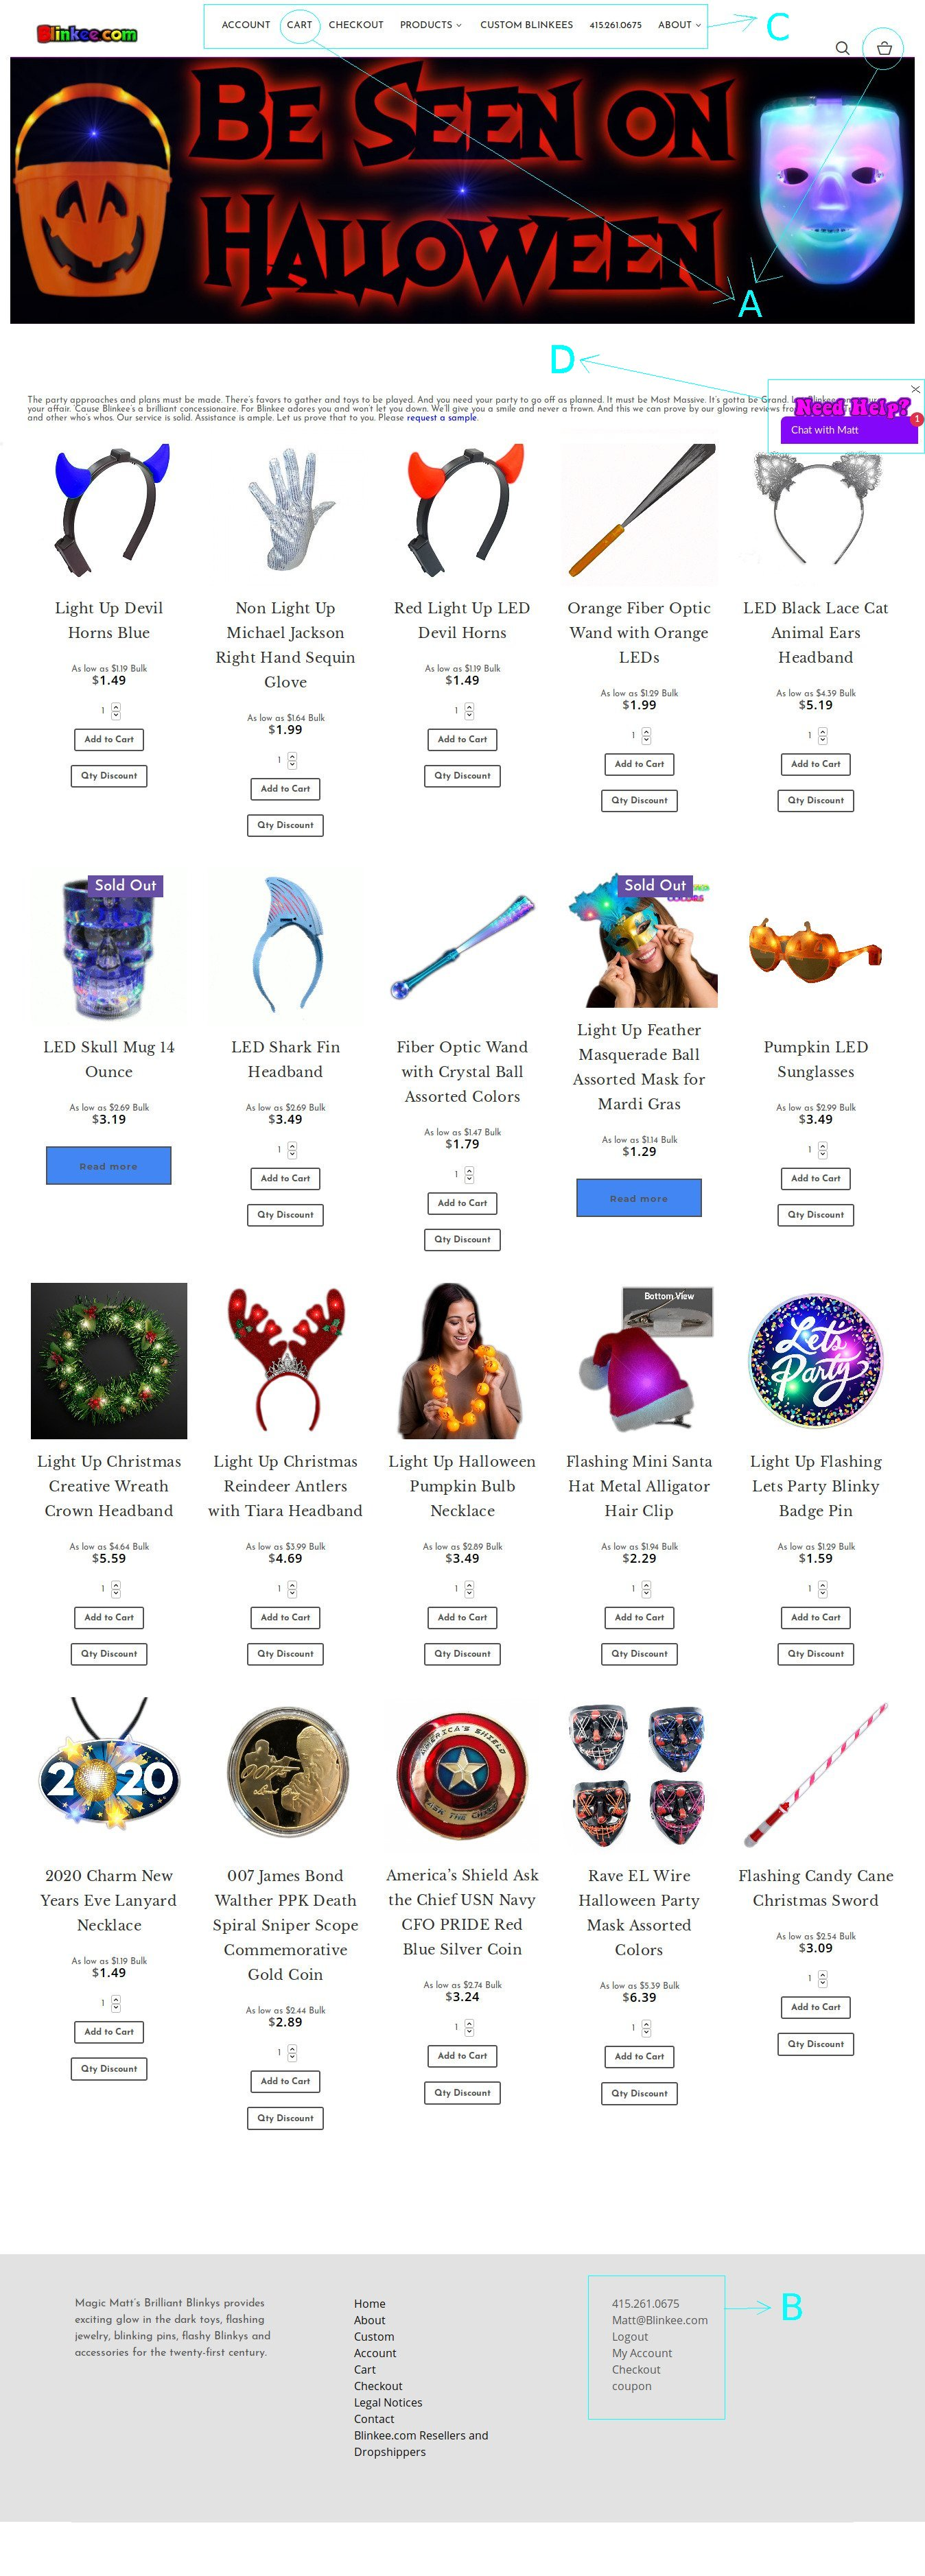
\includegraphics[clip, trim=0cm 109cm 0cm 0cm, scale=0.33]{./images/blinkee.jpg}
	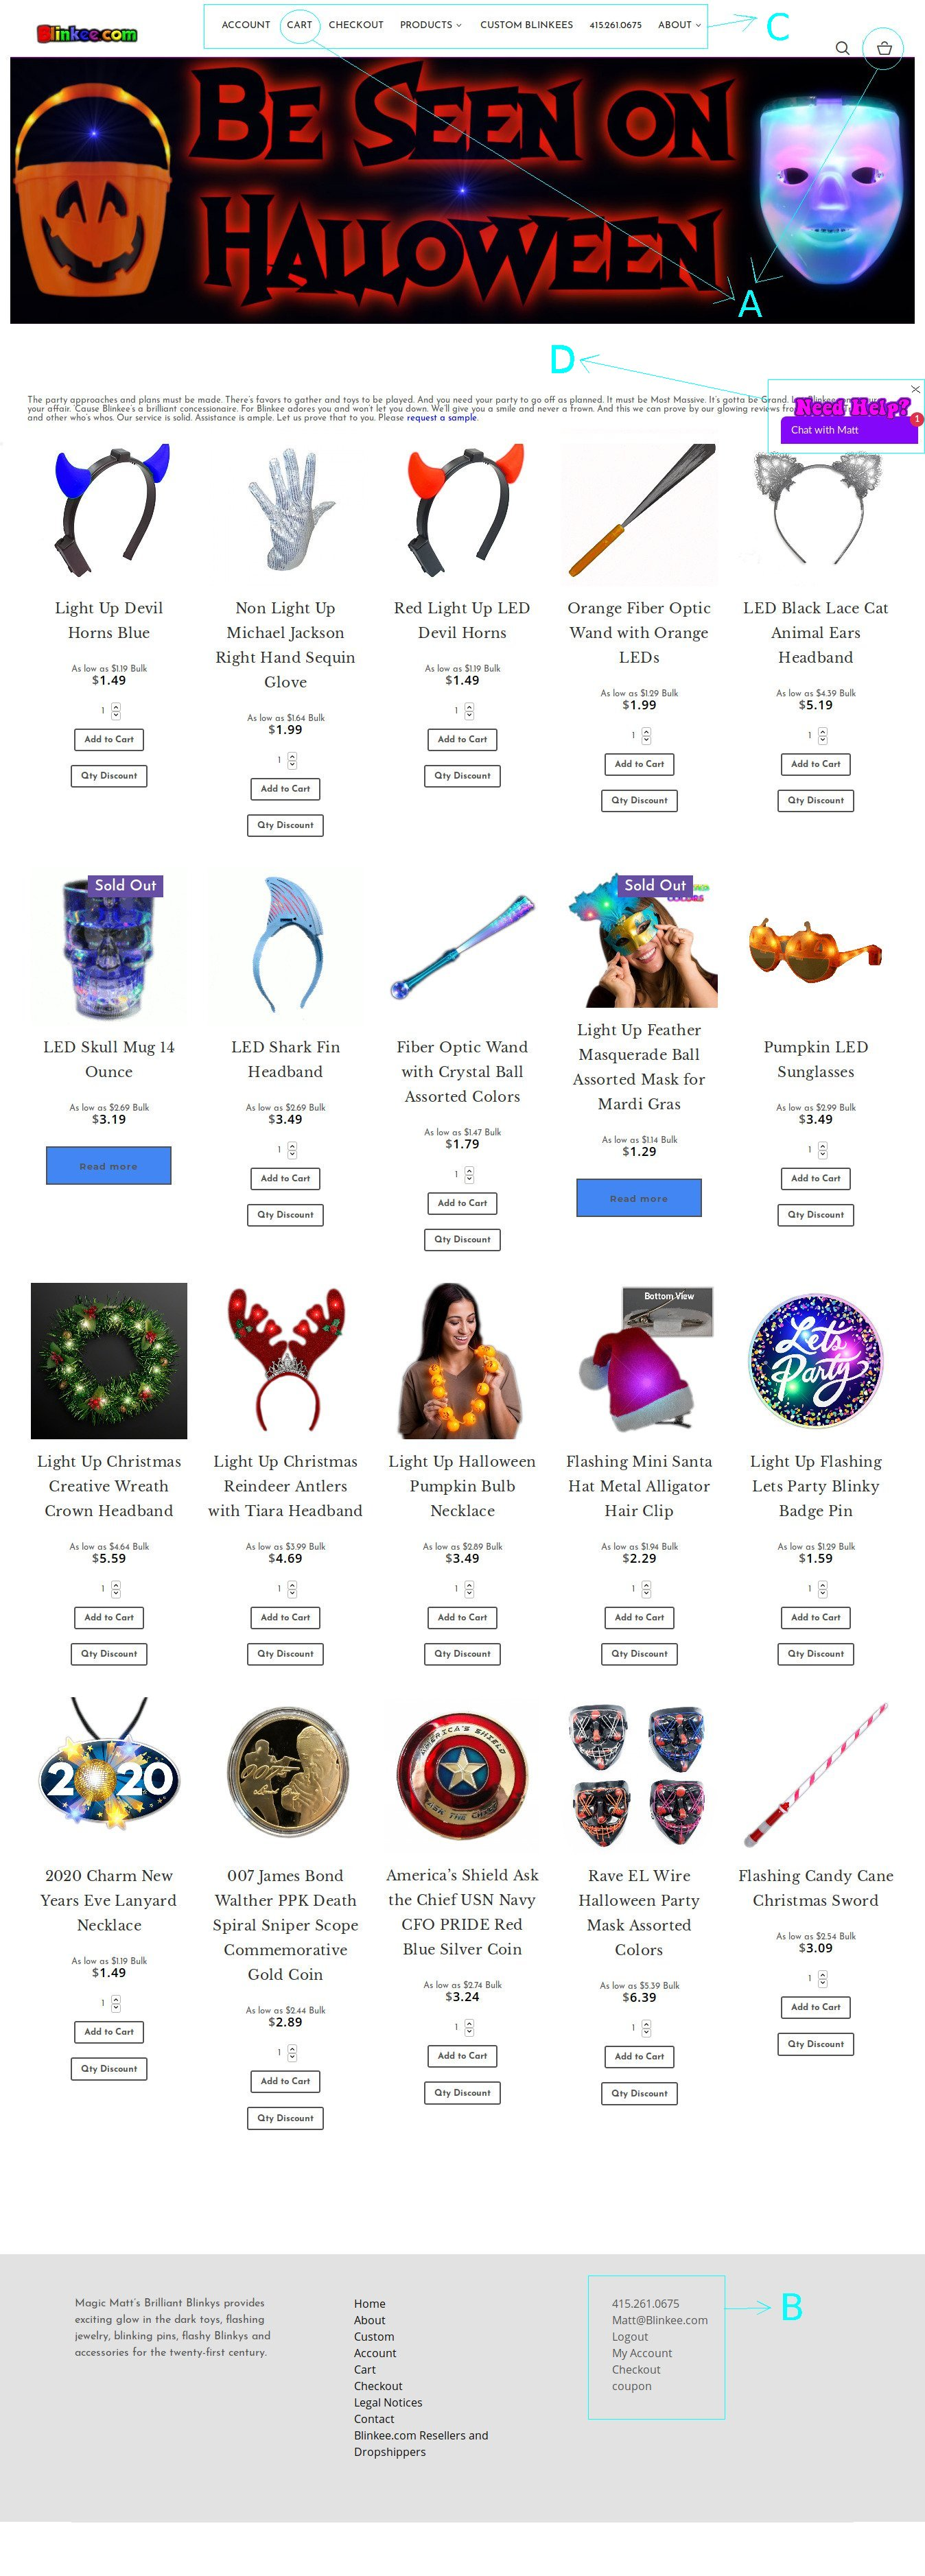
\includegraphics[clip, trim=0cm 8cm 0cm 117cm, scale=0.33]{./images/blinkee.jpg}
	\caption{Blinkee}
	\label{fig:sub2}
\end{figure}




\clearpage
\begin{tabularx}{\textwidth}{|X|}
	\hline
	\textbf{Applications of Design Elements}\\
	\hline
	\textbf{{[Law 1 (Good Shape) - positive]:}} figure \textbf{Gmail:A} has a shape of oval, which has a simple curvature, and thus, easy to remember.\\
	\hline
	\textbf{{[Law 3 (Closure) - positive]:}} \textbf{figure Gmail:B} shows that although not explicitly, the navigation bar on the left side is "hiddenly" closed. There is no visible line dividing this bar and the rest of the webpage, but those navigation buttons for different e-mail categories are perceived to be closed in a rectangular shape (also take note of different colouring than actual e-mail list tab).\\
	\hline
	\textbf{{[Law 6 (Experience) - positive]:}} \textbf{figure Gmail:C} makes use of two commonly used symbols, which even could be called universally acknowledged ones, one for "Social" segment (two people, one in front of the other), and one for "Promotions" segment (discount tag).\\
	\hline
	\textbf{{[Law 2 (Proximity) - negative]:}} \textbf{Blinkee:A} Cart tab and Cart sign both direct to the same URL, yet they are not packed or placed together, making the interface un-simple (if such a word exists). \\
	\hline
	\textbf{{[Law 4 (Similarity - negative)]:}} \textbf{Blinkee:C} topmost center buttons having no similarity (they having no indicative boundary too) does NOT help observing them as a group; they appear as individual parts while they are actually a part of navigation bar to help user traverse the website. This is not a good design.\\
	\hline
\end{tabularx}

\bigskip

\bigskip

%\begin{tabularx}{\textwidth}{|X|}
%	\hline
%	\textbf{Bad}\\
%%	\hline
%%	\textbf{{[Law 6 (Experience)]:}} \textbf{PaulGraham:A} and \textbf{PaulGraham:C} indicates that the navigation bar on the left is inconsistent. While homepage has missing "Home" button, "Essays" page has missing button of "Email". This inconsistency  \\
%	\hline
%	\textbf{{[Law 6 (Experience)]:}} \textbf{Blinkee:C} pressing cross button on the "Need Help" sign does not close the "Chat with Matt" part, it stays still. In this perspective, a user expects the duty of cross button to be to close the related part, which is not the case here.\\
%	\hline
%	
%	\textbf{{[Law 3 (Closure)]:}} \textbf{Blinkee:B} the objects sold have no closure at all. While overdone closures are repulsive, having none in this case does make it harder to connect objects with their properties such as the prices and the buttons. \\
%	\hline
%	\textbf{{[Law 1 (Good Shape)]:}} \textbf{Blinkee:B} makes use of no shapes, no boundaries in any of the DOM of the website. Not exploiting the cognitive compression, not in a slightest bit is a bad design. \\
%	\hline
%	
%\end{tabularx}

\bigskip

\bigskip

\textbf{Visibility}: + sign in "+ Compose" button at the top left of  \textbf{Gmail:A} is an example of visibility (we also mentioned about this in intentional signifier part). + sign conveys the idea of creating, and with its colors, it increases visibility of Compose button.\\


\textbf{Perceived affordance}: checkboxes in \textbf{Gmail:D} conveys the idea that I can interact with them to select multiple e-mails and operate on them at once.\\

\textbf{False affordance}: Logout button available although no login has been done (that it is not possible to logout without logging in first, thus, a false 'affordance') in \textbf{Blinkee:B}.\\



\textbf{Intentional signifier}: + sign in "+ Compose" button at the top left of  \textbf{Gmail:A} is a signifier. (although we have a distinct button for Compose, + sign is one of the few colored items in this webpage, and + sign signifies that I can create something, thus, and intentional signifier gathering attendance to its place)\\

\textbf{Misleading signifier}: "Need Help" box has a cross symbol when hovered over. What a user would expect is that it would get rid of "Need Help" \& "Chat with Matt" parts. However, clicking this button only get rids of "Need Help" part, leaving "Chat with Matt" part intact, which is a misleading signifier. (as two parts are together spatially, one expects that it would close both part, but it does not, and both parts are about helping, which does not furthermore help) in \textbf{Blinkee:D}.


\clearpage

\section*{Task 2}

\end{document}}
